\documentclass{standalone}
\usepackage{tikz}
\usepackage{amsmath}
\usepackage{graphicx}
\usetikzlibrary{positioning, shapes.geometric, shapes.multipart, arrows.meta, calc, fit}

% Global layout controls
\def\mainNodeSep{0.95cm}
\def\rowGap{0.42cm}
\def\colGap{0.9cm}
\def\legendOffsetX{1.2cm}
\def\legendPanelW{14.8cm}
\def\legendPanelH{10.2cm}
\def\legendPadX{0.6cm}
\def\legendTopInset{1.6cm}
\def\legendBottomInset{1.0cm}
\def\curveRound{5pt}

\newcommand{\MMMLSharedStyles}{
  \tikzset{
    basebox/.style={
      rectangle,
      rounded corners=2.5pt,
      draw=black!70,
      minimum height=0.95cm,
      minimum width=2.1cm,
      align=center
    },
    dense/.style={basebox, fill=orange!25,  minimum height=1.0cm, minimum width=1.2cm, text width=1.9cm},
    process/.style={dense},
    process2/.style={basebox, fill=orange!15, minimum height=0.8cm, text width=3.9cm},
    silu/.style={
      circle, draw=black!70, fill=white, minimum size=1.0cm,
      path picture={
        \draw[-, line width=0.9pt] (path picture bounding box.center) circle (0.28cm);
        \begin{scope}
          \clip (path picture bounding box.center) circle (0.28cm);
          \draw[-, domain=-2:2,smooth,variable=\x,line width=0.7pt]
            plot ({0.11*\x},{0.11*(\x/(1+exp(-\x)))});
        \end{scope}
      }
    },
    plusop/.style={
      circle, draw=black!70, fill=white, minimum size=1cm,
      path picture={
        \draw[-, line width=0.9pt]
          (path picture bounding box.west) -- (path picture bounding box.east);
        \draw[-, line width=0.9pt]
          (path picture bounding box.south) -- (path picture bounding box.north);
      }
    },
    basis/.style={basebox, fill=cyan!25, minimum height=1.0cm, minimum width=3.2cm},
    message/.style={basebox, fill=green!30, minimum height=1.2cm, minimum width=4.2cm},
    tensor/.style={basebox, fill=red!25, minimum height=1.2cm, minimum width=2.2cm},
    extra/.style={basebox, fill=gray!25, minimum height=1.2cm, minimum width=2.2cm},
    embedding/.style={basebox, fill=blue!25, minimum height=1.2cm, minimum width=4.2cm},
    output/.style={basebox, fill=yellow!25, minimum height=0.95cm, minimum width=0.8cm, align=center, font=\sffamily\Large},
    legendbox/.style={rectangle, draw=black!60, rounded corners=1.5pt, minimum width=0.8cm, minimum height=0.55cm},
    legendtext/.style={anchor=west, font=\sffamily\Large, align=left, text width=12.8cm}
  }
}


\begin{document}
\resizebox{\textwidth}{!}{%
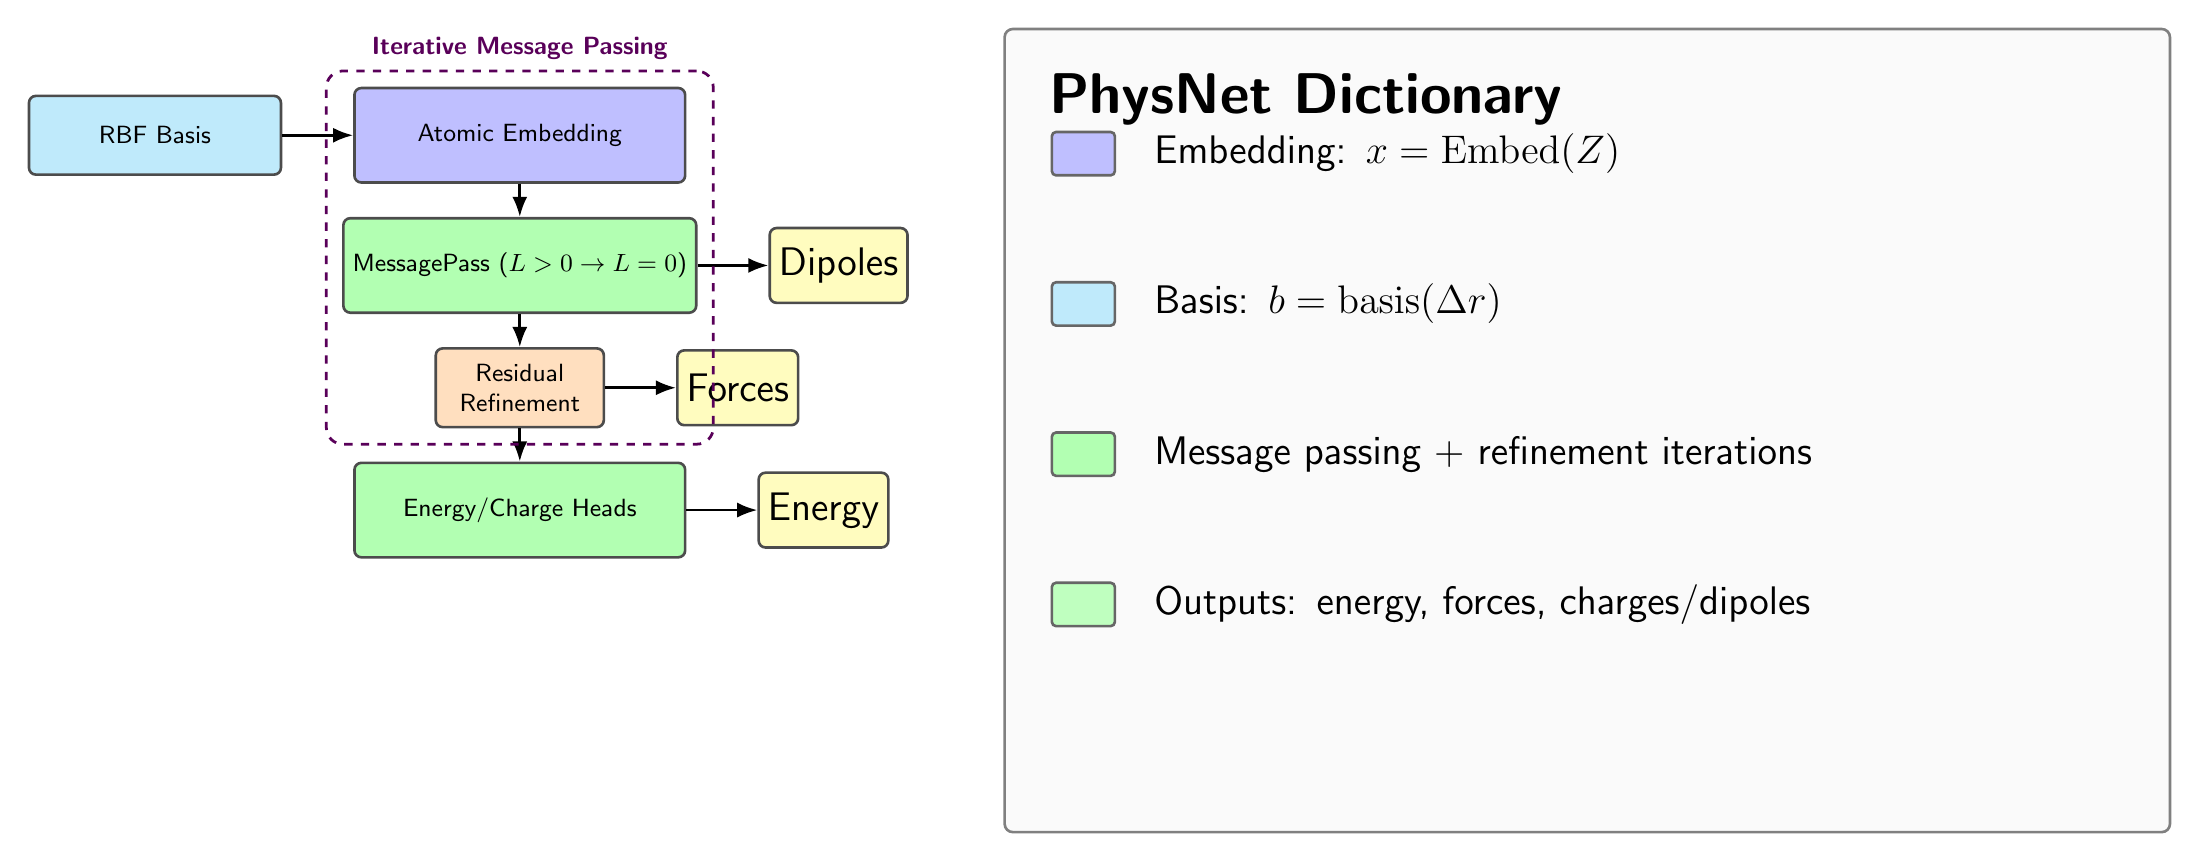
\begin{tikzpicture}[
  auto,
  node distance=\mainNodeSep and \mainNodeSep,
  line width=0.95pt,
  >=Latex,
  ->,
  font=\sffamily\small
]
  \MMMLSharedStyles

  \node[embedding] (embed) {Atomic Embedding};
  \node[basis, left=\colGap of embed] (basis) {RBF Basis};
  \node[message, below=\rowGap of embed] (mp) {MessagePass ($L>0 \rightarrow L=0$)};
  \node[dense, below=\rowGap of mp] (refine) {Residual Refinement};
  \node[message, below=\rowGap of refine] (head) {Energy/Charge Heads};
  \node[output, right=\colGap of head] (energy) {Energy};
  \node[output, right=\colGap of refine] (forces) {Forces};
  \node[output, right=\colGap of mp] (dipoles) {Dipoles};

  \draw[->] (basis.east) -- (embed.west);
  \draw[->] (embed) -- (mp);
  \draw[->] (mp) -- (refine);
  \draw[->] (refine) -- (head);
  \draw[->] (head) -- (energy);
  \draw[->] (refine) -- (forces);
  \draw[->] (mp) -- (dipoles);

  \node[draw=violet!70!black, rounded corners=6pt, dashed, line width=1.0pt, inner sep=0.2cm,
    fit=(embed) (mp) (refine)] (loop) {};
  \node[anchor=south, font=\sffamily\small\bfseries, text=violet!70!black] at (loop.north) {Iterative Message Passing};

  \path (current bounding box.north east) coordinate (figNE);
  \node[draw=black!50, rounded corners=3pt, fill=black!2, minimum width=\legendPanelW, minimum height=\legendPanelH, anchor=north west]
    (legendpanel) at ($(figNE)+(\legendOffsetX,0)$) {};
  \coordinate (legStart) at ($(legendpanel.north west)+(\legendPadX,-\legendTopInset)$);
  \coordinate (legEnd) at ($(legendpanel.south west)+(\legendPadX,\legendBottomInset)$);
  \coordinate (leg2) at ($(legStart)!0.25!(legEnd)$);
  \coordinate (leg3) at ($(legStart)!0.5!(legEnd)$);
  \coordinate (leg4) at ($(legStart)!0.75!(legEnd)$);

  \node[anchor=north west, font=\sffamily\bfseries\huge] at ($(legendpanel.north west)+(0.45,-0.45)$) {PhysNet Dictionary};
  \node[legendbox, fill=blue!25, anchor=west] (lg1) at (legStart) {};
  \node[legendtext, right=0.35cm of lg1.east, anchor=west] {Embedding: $x=\mathrm{Embed}(Z)$};
  \node[legendbox, fill=cyan!25, anchor=west] (lg2) at (leg2) {};
  \node[legendtext, right=0.35cm of lg2.east, anchor=west] {Basis: $b=\mathrm{basis}(\Delta r)$};
  \node[legendbox, fill=green!30, anchor=west] (lg3) at (leg3) {};
  \node[legendtext, right=0.35cm of lg3.east, anchor=west] {Message passing + refinement iterations};
  \node[legendbox, fill=green!25, anchor=west] (lg4) at (leg4) {};
  \node[legendtext, right=0.35cm of lg4.east, anchor=west] {Outputs: energy, forces, charges/dipoles};
\end{tikzpicture}%
}
\end{document}
